\clearpage
\section{典型例题与完整分析}
\label{sec:ch6-worked-examples}

\noindent 以下以 $f$ 表示Hz频率，DFT采用正变换不除以点数的约定；相关一律取 $R_{xy}(\tau)=\mathrm E[x(t)y(t+\tau)]$。解题时先分清采样频带、观察时长、幅值归一化与功率归一化，再代入数值。

\subsection{例题1：混叠判定与量化位数选择}
\keypoint{复习重点：直接代入采样时刻验证混叠，按完整输入跨度计算量化步长。}

\qs{两个频率为何变成一个频率}{模拟输入为
\[
x(t)=\cos(2\pi70t)+0.4\cos(2\pi130t)\quad(\mathrm V).
\]
以 $f_s=200\,\mathrm{Hz}$ 采样，求得到的序列及其可见频率；若需保留全部输入成分，采样率至少应满足什么条件？另有 $\pm5\,\mathrm V$ 的均匀ADC，要求未过载舍入量化误差不超过 $1\,\mathrm{mV}$，至少应选多少位？}

\sol
\textbf{先检查采样上限。}奈奎斯特频率为 $100\,\mathrm{Hz}$，$130\,\mathrm{Hz}$ 超过上限，其折叠频率为 $|130-200|=70\,\mathrm{Hz}$。代入 $t=n/200$，
\begin{align*}
\cos\left(2\pi\frac{130}{200}n\right)
&=\cos\left(2\pi n-2\pi\frac{70}{200}n\right)\\
&=\cos\left(2\pi\frac{70}{200}n\right).
\end{align*}
所以
\[
\boxed{x[n]=1.4\cos\left(2\pi\frac{70}{200}n\right)\quad(\mathrm V)}.
\]
数字记录呈现一条幅值为 $1.4\,\mathrm V$ 的 $70\,\mathrm{Hz}$ 余弦，无法从该记录单独恢复原来的两条成分。增加同一采样率下的记录长度或补零，都不能把它们分开。

若要保留最高 $130\,\mathrm{Hz}$ 的全部成分，理想低通采样应满足
\[
\boxed{f_s>260\,\mathrm{Hz}}.
\]
实际还要为抗混叠滤波器留出过渡带。若目标只保留 $70\,\mathrm{Hz}$ 成分，可在采样前抑制 $130\,\mathrm{Hz}$；这与采集后从混叠序列中分离两者是不同的任务。

\textbf{再求量化位数。}完整量程跨度 $D=5-(-5)=10\,\mathrm V$，采用 $\Delta_q=D/2^b$，要求
\[
\frac{\Delta_q}{2}=\frac{10}{2^{b+1}}\,\mathrm V\leq0.001\,\mathrm V
\quad\Longrightarrow\quad 2^b\geq5000.
\]
由于 $2^{12}=4096<5000$、$2^{13}=8192>5000$，故
\[
\boxed{b_{\min}=13},\qquad
\Delta_q=\frac{10}{8192}\,\mathrm V\approx1.2207\,\mathrm{mV},
\]
对应最大舍入误差约 $0.6104\,\mathrm{mV}$，满足要求。

\nt{\textbf{易错：}奈奎斯特频率为 $f_s/2$，不能把 $f_s$ 本身当作采样频带上限。量化要求约束的是半个LSB；13位是满足该量化模型的最低位数，并不等于整条测量链已具备 $1\,\mathrm{mV}$ 的总准确度。}

\Needspace{8cm}
\subsection{例题2：记录长度、泄漏与加零的区别}
\keypoint{复习重点：用 $f_0T$ 判断是否整周期，以实际采集时长解释分辨能力。}

\qs{102 Hz与500 Hz的有限记录}{以 $f_s=5120\,\mathrm{Hz}$、$N=1024$ 采集
\[
x(t)=\sin(2\pi102t)+\sin(2\pi500t).
\]
求 $T_s,T,\Delta f$，判断两成分是否落在DFT频点上。若补零到4096点，频点间距如何变化？若要在该采样率下使原始DFT间距不大于 $1\,\mathrm{Hz}$，至少需要多少个实际样本？}

\sol
四个基本量为
\[
T_s=\frac1{5120}\,\mathrm s=0.1953125\,\mathrm{ms},\quad
T=\frac{1024}{5120}=0.2\,\mathrm s,\quad
\boxed{\Delta f=5\,\mathrm{Hz}}.
\]
两条成分的频点序号分别为
\[
\frac{102}{5}=20.4,\qquad\frac{500}{5}=100.
\]
因此 $500\,\mathrm{Hz}$ 对应 $k=100$，记录中恰有100个周期；$102\,\mathrm{Hz}$ 记录中有20.4个周期，未落在频点上，会出现泄漏与峰值漏读。其最近的频点为 $k=20$，对应 $100\,\mathrm{Hz}$，直接读最大频点会产生约 $-2\,\mathrm{Hz}$ 的频率偏差。

\begin{center}
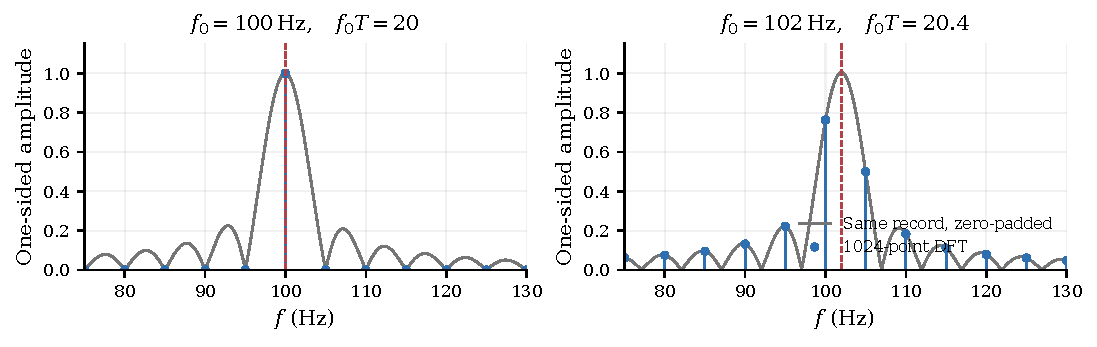
\includegraphics[width=.98\linewidth]{ch6-leakage.pdf}
\end{center}
图中把单频情况分开画出：左侧 $100\,\mathrm{Hz}$ 与本题的 $500\,\mathrm{Hz}$ 一样满足相干条件，右侧 $102\,\mathrm{Hz}$ 则不满足。蓝点为原始DFT，灰线为同一记录补零后的密集取值。对\textbf{单独的}单位幅值 $102\,\mathrm{Hz}$ 分量，原始100 Hz点的单边幅值约为 $0.7623$，小于真实幅值1；两频叠加时还需考虑各自泄漏的复数叠加。

补零后，
\[
\boxed{\Delta f_{\mathrm{grid}}=\frac{5120}{4096}=1.25\,\mathrm{Hz}}.
\]
但实际观察时长仍为 $0.2\,\mathrm s$，矩形窗主瓣零点间宽度仍约为 $2/T=10\,\mathrm{Hz}$。补零能更清楚地显示谱峰的位置，不能把原记录的有效时长改成 $0.8\,\mathrm s$。

要使\textbf{未补零的}DFT间距满足 $f_s/N\leq1\,\mathrm{Hz}$，应有
\[
\boxed{N\geq5120},\qquad \boxed{T\geq1\,\mathrm s}.
\]
取 $N=5120$ 时，两频均恰好落点，记录内分别有102与500个周期。若换成Hann窗，泄漏旁瓣较低，但主瓣约为矩形窗的两倍宽，实际可分辨的频率间隔仍需另行评估。

\nt{\textbf{易错：}“间距不大于1 Hz”给出的是频点要求，不保证任意相差1 Hz、幅值悬殊且含噪的两条成分都能分开。时标应取 $n/f_s$（$n=0,\ldots,1023$）；DFT频标应取 $kf_s/N$，不能用含 $f_s$ 终点的 $N$ 个等分点代替。}

\Needspace{8cm}
\subsection{例题3：用互相关时延测运动速度}
\keypoint{复习重点：先用延迟模型确认相关峰的正负，再把样本时移换成秒。}

\qs{两探头之间的传播时间}{两个探头沿带材运动方向依次布置，间距 $d=0.30\,\mathrm m$。前、后探头分别记录 $x[n]$ 和 $y[n]$，采样率均为 $f_s=20\,\mathrm{kHz}$。已知表面特征在两探头间近似不变，在允许时延范围内，按 $\sum_nx[n]y[n+\ell]$ 定义的互相关主峰位于 $\ell=+120$。求运动速度，并说明交换两信号顺序后峰位如何变化。}

\sol
带材先经过前探头，后探头记录为延迟副本，可写成
\[
y(t)=a\,x(t-\tau_d)+n(t),\qquad a>0,
\]
其中 $n$ 为与 $x$ 不相关、零均值的测量干扰。采用本章约定，
\[
R_{xy}(\tau)=aR_x(\tau-\tau_d),
\]
故正侧峰对应后探头信号晚到，和物理顺序一致。峰位的实际时延为
\[
\boxed{\tau_d=\frac{120}{20000}=0.006\,\mathrm s=6\,\mathrm{ms}}.
\]
两探头之间是单程运动距离，因此
\[
\boxed{v=\frac{d}{\tau_d}=\frac{0.30}{0.006}=50\,\mathrm{m/s}}.
\]
若改算 $R_{yx}$，由 $R_{yx}(\tau)=R_{xy}(-\tau)$，主峰在 $\ell=-120$，时延大小与速度不变。若误把此时延当成雷达往返时间再除以2，就会得到错误结果。

若另有依据保证峰位误差不超过 $\pm1$ 个样本，且暂不计探头距离误差，则速度范围为
\[
\frac{0.30\times20000}{121}\leq v\leq
\frac{0.30\times20000}{119},
\qquad \boxed{49.59\lesssim v\lesssim50.42\,\mathrm{m/s}}.
\]
这只是给定峰位误差界下的换算；不能仅从 $T_s=50\,\mu\mathrm s$ 就断定实际时延误差必然为一个样本。

\nt{\textbf{易错：}相关峰的符号依赖信号顺序和时移定义；周期特征还会产生多个候选峰，应利用几何关系与速度范围选峰。只有两探头观察同一随动特征且变形较小时，$v=d/\tau_d$ 才有明确含义。}

\Needspace{8cm}
\subsection{例题4：同频相关、相位差与线功率谱}
\keypoint{复习重点：自相关不含绝对初相位，互相关保留相对相位；谱线权重代表功率。}

\qs{正弦信号的相关与功率}{设
\[
x(t)=2\sin(100\pi t+\theta),\qquad
y(t)=3\sin(100\pi t+\theta-\pi/3).
\]
按长期时间平均求 $R_x(\tau),R_y(\tau),R_{xy}(\tau)$，给出最小正互相关峰位置，并写出 $x$ 的双边功率谱与有效值。}

\sol
两信号频率为 $f_0=50\,\mathrm{Hz}$，周期 $T_0=0.02\,\mathrm s$，均值均为零。利用
\[
\sin\alpha\sin\beta=\frac12[\cos(\alpha-\beta)-\cos(\alpha+\beta)],
\]
一周期平均后，含 $2\omega_0t$ 的余弦项为零，留下
\[
\boxed{R_x(\tau)=2\cos(100\pi\tau)},\qquad
\boxed{R_y(\tau)=\frac92\cos(100\pi\tau)}.
\]
互相关为
\begin{align*}
R_{xy}(\tau)
&=\frac1{T_0}\int_0^{T_0}2\sin(100\pi t+\theta)
\,3\sin[100\pi(t+\tau)+\theta-\pi/3]\diff t\\
&=\boxed{3\cos(100\pi\tau-\pi/3)}.
\end{align*}
绝对初相位 $\theta$ 在平均后消失，相对相位 $\pi/3$ 留在互相关中。归一化结果为 $\rho_{xy}(\tau)=\cos(100\pi\tau-\pi/3)$。

峰值条件是 $100\pi\tau-\pi/3=2\pi m$，故
\[
\tau=\frac1{300}+m\times0.02\quad(\mathrm s),\qquad m\in\mathbb Z.
\]
最小正峰为 $\boxed{\tau_d=3.333\,\mathrm{ms}}$，但它与任意相差整数个周期的时延产生相同的周期波形，因此不能在无其他先验时宣称时延已唯一确定。

由 $\cos(2\pi f_0\tau)\leftrightarrow\tfrac12[\delta(f-f_0)+\delta(f+f_0)]$，
\[
\boxed{S_x(f)=\delta(f-50)+\delta(f+50)}.
\]
每条双边谱线权重为1，总功率为2，与 $R_x(0)=2$ 一致，故
\[
\boxed{x_{\mathrm{rms}}=\sqrt2},\qquad
G_x(f)=2\delta(f-50)\quad(f>0).
\]
单边谱线权重2等于该正弦的均方值 $A^2/2$，不是峰值幅度2的另一种写法。这里两者恰巧数值相同，物理量与量纲仍不同。

若把 $y$ 的频率改为与50 Hz不同的正频率，两个零均值正弦的长期互相关为零；有限记录内的积分一般仍会有残差，不能据此把有限样本互相关一律置零。

\Needspace{8cm}
\subsection{例题5：从DFT核对PSD面积与有效值}
\keypoint{复习重点：频点上的PSD值需乘频宽后求和，内部单边频点合并负频率功率。}

\qs{四点余弦的周期图}{采样率 $f_s=4\,\mathrm{Hz}$，记录为
\[
x[n]=[1,\ 0,\ -1,\ 0]\quad(\mathrm V),\qquad n=0,1,2,3.
\]
采用矩形窗和未归一化DFT，计算双边、单边PSD，并核对平均功率。若数据补零到16点，应怎样改变PSD计算？}

\sol
本记录是 $1\,\mathrm{Hz}$ 单位幅值余弦的一个完整周期，$N=4$、$T=1\,\mathrm s$、$\Delta f=1\,\mathrm{Hz}$。DFT为
\[
X_4[k]=1-e^{-\iu\pi k}=[0,\ 2,\ 0,\ 2].
\]
其中 $k=3$ 表示 $f=-1\,\mathrm{Hz}$，不是一条独立的 $3\,\mathrm{Hz}$ 模拟成分。双边周期图的分母为 $Nf_s=16$，得到
\[
\boxed{\widehat S_x(f_k)=[0,\ 0.25,\ 0,\ 0.25]\quad(\mathrm{V^2/Hz})}.
\]
频率0、1、2 Hz的单边谱为
\[
\boxed{\widehat G_x=[0,\ 0.50,\ 0]\quad(\mathrm{V^2/Hz})}.
\]
只有1 Hz内部点加倍，直流和2 Hz奈奎斯特点不加倍。谱面积为
\[
\sum_k\widehat S_x(f_k)\Delta f
=(0.25+0.25)\times1=0.5\,\mathrm{V^2},
\]
单边谱也给出 $0.50\times1=0.5\,\mathrm{V^2}$。时域核对为
\[
\frac14\sum_{n=0}^{3}x^2[n]=\frac{1+0+1+0}{4}=0.5\,\mathrm{V^2},
\qquad \boxed{x_{\mathrm{rms}}=\frac1{\sqrt2}\,\mathrm V}.
\]
这与正弦有效值公式一致。

补零到 $M=16$ 点后，频点间距改为 $f_s/M=0.25\,\mathrm{Hz}$，但实际窗仍只有4个非零样本，故
\[
\boxed{\widehat S_x(f_k)=\frac{|X_{16}[k]|^2}{16}},\qquad
\boxed{\sum_{k=0}^{15}\widehat S_x(f_k)\times0.25=0.5\,\mathrm{V^2}}.
\]
新的密集频点展示有限记录的连续谱形；不能误用 $Mf_s=64$ 作分母，否则谱面积会缩小为原来的四分之一。

\nt{\textbf{易错：}PSD纵坐标与功率不是同一个量；只有乘上对应频宽并累加，才得到均方值。这里频宽恰为1 Hz，使二者数值看似相同；换一个记录长度，就不能再凭数值巧合判断。}
